\documentclass{article}
\usepackage{blindtext}
\usepackage{titlesec}
\usepackage[utf8]{inputenc}
\usepackage[parfill]{parskip}
\usepackage{algorithm}
\usepackage{algorithmic}
\usepackage{graphicx}

\usepackage{hyperref}

\begin{document}
\begin{titlepage}
    \begin{center}
        \vspace*{1cm}
        \Huge
        \textbf{Quantum particles in fractal external potential}

        \vspace{0.5cm}
        \Large
        GEP Final Deliverable
        \vfill
        \begin{figure}[h!]
            
\includegraphics[width=\textwidth]{./logo-fib.png}
        \end{figure}
        \textbf{Marc Amorós}\\
        \vspace{0.5cm}
        \textbf{Thesis supervisor: Grigori Astrakharchik}\\
        \vspace{0.5cm}

   \end{center}
\end{titlepage}

\tableofcontents
\break

\section{Context}
\subsection{Introduction}
The investigation world is always closely related to computer science. It is very frequent to solve a problem by modelling it on a computer using a certain programming language, and then making simulations to get a solution.\\

The physics investigation field highly benefits of this problem-solving approaches, as we find plenty of equations with physical meaning without an exact solution. To fix this, we try to solve them by representing these equations in a discrete and finite way, so our computers can handle it, and then we write algorithms to get approximations of a real solution.\\

This is an interdisciplinary research project, with an important theoretical part that involves some physics knowledge and a practical part that covers the design and development of algorithms to simulate and solve quantum physics systems.\\

\subsection{Stakeholders}
It is important to define the stakeholders of any project, to know who is interested of its development and can benefit from it.\\

The main stakeholder of this project is UPC physics department, and more concretely Grigori Astrakharchikm, who was the impeller of it, by posting a TFG offer on Racó. This can lead to a scientific publication if interesting results are obtained, that is why it can interest him as a researcher.\\

As every scientific research project, it increases the knowledge on this field in general. If we write a paper about the steps we followed it can be beneficial for any other researcher of quantum particle systems and their properties, even they could try to replicate our results by real experimentation. So it can be considered that this project benefits all the scientific community in a way, more specifically the physics investigators.  

\subsection{Theoretical concepts}
I will summarize some theoretical concepts that are necessary to understand the rest of this document, so the reader can fully comprehend the aim and objectives of this project.

\subsubsection{Quantum mechanics}
Quantum mechanics is the theory that describes the physical properties of Nature at the scale of atoms and subatomic particles. When it was first formulated during the early decades of the 20th century, it introduced some ground-breaking concepts such as energy quantization, the uncertainty of position and momentum of a particle and the wave-particle duality of matter.\\

In classical physics we have Newton’s second law, which given a set of initial conditions it can make a mathematical prediction of what path a given physical system will take over time. Its quantum analogous would be the Schrödinger equation which instead requires a statistical interpretation.

\subsubsection{Schrödinger equation}
Quantum mechanics tells us how the particles behave over time. This description is done using the Schrödinger equation, which provides the time evolution of the wavefunction ($\Psi$) of particles. The wavefunction is a mathematical description of the quantum state of the system, and with it, you can obtain the distribution of probability of the measurements that you can do over this system.\\

The Schrödinger equation is a differential equation, and has the following form:

\begin{equation}
i\hbar\frac{\partial}{\partial t}\Psi\left(r,t\right)=\hat{H}\Psi\left(r,t\right)
\end{equation}
Here we define the Hamiltonian operator $\hat{H}$, which is an operator corresponding to the total energy of that system, including both kinetic ($T$) and potential energy ($V$), and for a single particle it takes the form:
\begin{equation}
\hat{H}=\hat{T}+\hat{V}=-\frac{\hbar^2}{2m}\nabla^2+V\left(\mathbf{r},t\right)
\end{equation}
The kinetic energy in quantum mechanics is proportional to the Laplace operator $\nabla^2$, which is the addition of the second partial derivatives of the wavefunction. The potential energy is a function of the position of the particle, similarly to the classical case.\\

We are interested in the stationary properties, so we take the time-independent version of the Schrödinger equation:
\begin{equation}
\hat {H} |\Psi \rangle = E |\Psi \rangle
\end{equation}
When solving it, the set of energy eigenvalues that provides (also called energy spectrum) is the set of possible energies obtained when measuring the system’s total energy. Here we are interested in finding the ground state of the system, which is its lowest energy state. Differently from the classical systems where the energy of a single particle at zero temperature is finite due to zero-point motion, this ground state energy is always present in the quantum system, even in absolute zero temperature conditions. 

\subsubsection{Bose–Einstein condensate and Gross–Pitaevskii equation}
Bose–Einstein condensate \cite{BEC} (BEC) is a state of matter which occurs when a gas of bosons is cooled down to nearly the absolute zero. Under such conditions, a macroscopic fraction of bosons occupy the ground state and the whole system can be described by the same wavefunction. Such a wavefunction satisfies the Gross–Pitaevskii equation, which describes the ground state of a quantum system of identical bosons. 

\subsubsection{Fractals}
A fractal is a subset of the Euclidean space that illustrates a property called self-similarity, which means that appears the same at different scales and exhibits similar patterns at increasingly smaller scales. 

\subsubsection{Sierpiński carpet}
The Sierpiński carpet is a plane fractal that was first described by Wacław Sierpiński in 1916, as a two dimensions generalization of the Cantor set, that was discovered in 1874 by Henry John Stephen Smith and introduced by German mathematician Georg Cantor in 1883.\\

The Cantor ternary set is created by iteratively deleting the open middle third from a set of line segments.

\begin{figure}[h]
    
\includegraphics[width=\textwidth]{./cantor.png}
    \caption{First six steps of Cantor ternary set}
\end{figure}
\begin{figure}[h]
    \centering
    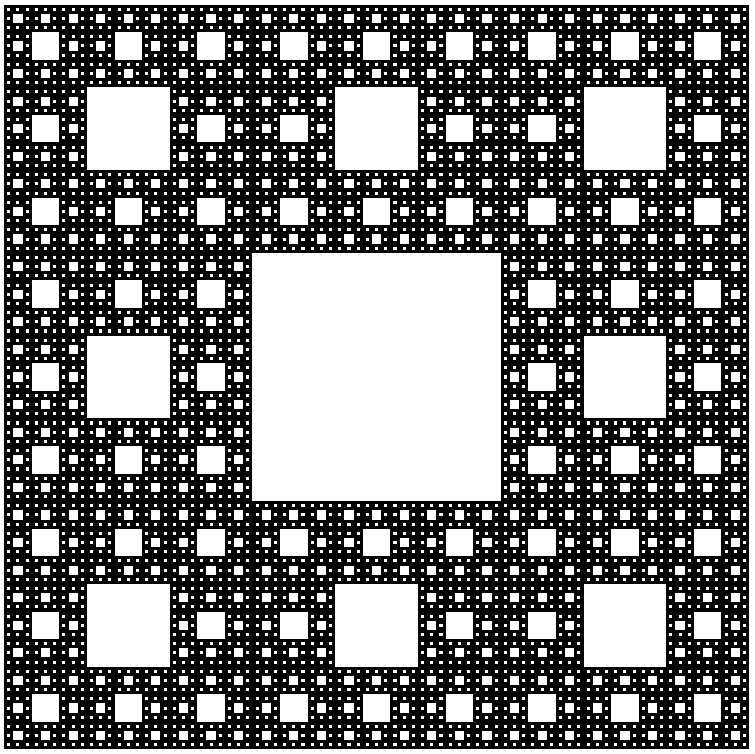
\includegraphics[scale=0.4]{./sierpinski.png}
    \caption{Sierpiński carpet with 5 levels of recursion}
\end{figure}
\vfill
\section{Justification}
The interdisciplinary aspect of this project is what attracts me the most. Quantum mechanics is a complicated field that we do not study on the GEI degree. That is why this project really interested me personally, as it gives me the opportunity to learn and work on a subject that is quite different to what I am used to, and I am also able to contribute on a physics research project applying my computation knowledge, something I would enjoy doing as a future job.\\

There have been recent experiments \cite{boseeinstein} that have shown how it is possible to produce a Bose-Einstein condensate. In the last few years, new experimental techniques have been developed, and it became feasible to create two-dimensional Fermi or Bose gas in highly controllable external potential. The projected potential can be chosen essentially in any desired shape, fractal shapes included. This means that our work could be verified by experimentation.

\section{Objectives}
The aim of the project is to study the properties of quantum particles in a fractal external potential. The main goal is to obtain a detailed description of such a system in terms of energetic, structural and dynamic properties. In particular, the energetic properties can be quantified by evaluation of the ground state energy and the excitation spectrum. The structural property of interest is the density profile. The dynamic property to be calculated is the diffusion coefficient.\\

We consider the external potential in the shape of a Sierpiński carpet. It has a fractal structure with the fractal dimensionality between 1 (i.e. a line) and 2 (i.e. a plane). The strength of the external potential is considered to be infinite (i.e. hard walls) in the positions where the fractal is present. It means that the particles cannot diffuse freely in the system. At the same time, the phase space is joined, that is the particle is allowed to move between any two points where the external field is absent. The fractal shape is defined in a simple recursive procedure and depends on the recursion level. \\

One of our goals is to provide a detailed description of the properties of quantum particles in fractal external potential. In particular, we plan to verify the existence of a simple scaling law between the recursion number of the zero-point energy of the system and the number of iterations of the fractal.\\

This is an interdisciplinary problem, based on application of mathematical concepts to the field of quantum physics, and relies on the use of numerical methods. This project requires carrying out a scientific investigation and a priori it is not clear which quantum system is going to be the best to study these properties.

\section{Scope}
We plan to execute this study considering different types of atoms confined to an external fractal potential. In particular we will consider:
\begin{itemize}
    \item One quantum particle 
    \item Ideal Fermions
    \item Interacting Bosons
\end{itemize}

In this way we cover the major typical experimental conditions. In experiments with ultracold atoms, the atoms obey either Bose-Einstein statistics (bosons) or Fermi-Dirac statistics (fermions). A proper simulation of the properties requires an implementation of different methods used to address the system's properties such as:
\begin{enumerate}
    \item Exact diagonalization technique, applicable to one particle and many-body system composed of fermions.
    \item Random Walk stochastic method, applicable to one particle.
    \item Gross-Pitaevskii equation, applicable to many-body system composed of bosons.
\end{enumerate}
Method 1 allows to obtain energetic and structural properties, while method 2 the structural and dynamic ones. Method 3 can be used to obtain energetic, structural and dynamic properties of the system.


\section{Potential obstacles and risks}
The biggest obstacle to me is the fact that I have to really comprehend all the physical concepts to be able to properly implement the techniques to model and solve the quantum systems that we propose. I am a computer science student and I have not been taught quantum mechanics, what means that this project involves a lot of self-studying by my part.\\

Another obstacle/risk is the possibility that some of the systems that we propose are not good to observe the properties we are searching for. That is why we want to try different quantum systems and compare the viability of studying them when applying an external field with a fractal shape.

\section{How the project will be developed}
As our goal is to study the effect of the external potential field on a quantum system, we must compute the ground state energy of the quantum system that we present. \\

To do so, for the case of a single particle in an infinitely high external potential box mathematically described by zero boundary conditions, we must solve the time-independent Schrödinger equation while we apply the external potential field to the box. We implement a Matlab code that generates a Sierpiński carpet given a recursion number and we apply the field to the particle by defining the potential energy part of the Hamiltonian operator using this fractal. This potential is described by the function $V(x, y)$ ,which checks if the position $(x, y)$ of the fractal is filled or empty. With this done, we solve the time-independent Schrödinger equation on a discretized two-dimensional space, and we obtain the ground state energy and the wavefunction of the particle. In Figure 3 it can be seen the wavefunction obtained as a result of first experiments using this method.\\

\begin{figure}[h]
    \centering
    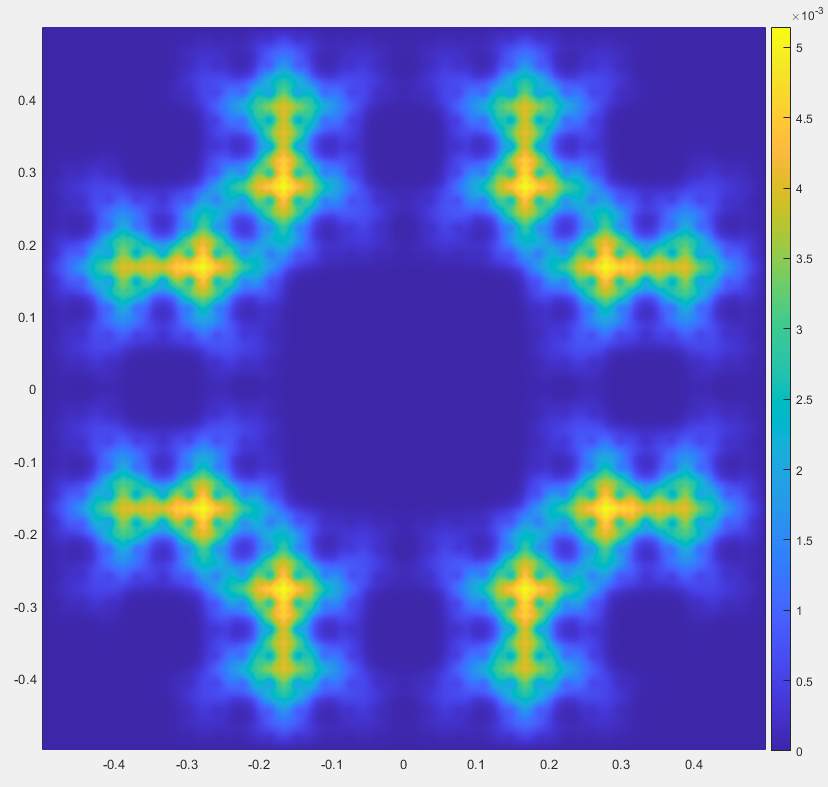
\includegraphics[scale=0.5]{./wavefunction.png}
    \caption{Wavefunction of a particle in a box with Sierpinski shaped external potential}
\end{figure}

We are going to repeat this process using a different number of iterations of the fractal, so we can deduce the relation that this parameter has with the zero-point energy. \\

We want to obtain a result, and as memory and computation resources are limited, we must define some discretization of the space that reflects in a computable problem. An option is to solve the problem with different values for $N$ (being $N$ the number of fractions the space is divided in) and study how this evolves when $N$ goes to infinity, or analogously, when $1/N$ goes to 0.\\

As this first case involves a relatively simple quantum system, we can define a way of obtaining an exact solution of the system's properties that we are interested in. But as I previously mentioned on this document, there are a lot of systems without exact solutions, as we do not know how to solve them. To handle this, we are going to use numerical methods such as random walks to approximate solutions for the system's properties.
\vfill
\break
\subsection{Methodology and rigour}
As this is a research project, every step we take is going to be vastly justified. Every modelling of a system is going to be verified by computing some properties that we know in advance, such as that the ground energy of a particle in a box without an external potential has to be equal to $\frac{\pi^2\hbar}{2mL^2}$. Also, all the techniques followed to model and solve the systems are going to be referenced and explained in detail on the thesis documentation. 

Scrum is a working methodology really adequate for a complex project, such as ours, as we do not really know everything we are going to encounter when previously planning, and this methodology allows us to keep revising the steps to follow every sprint. This gives us the ability to react to the unexpected problems we may bump into. The sprints are going to bee one week long and every Tuesday we are going to meet for a sprint review and to plan the next weeks tasks.

\section{Project phases}
To achieve the aim of the project, that is to study the properties of quantum particles in a fractal external potential, we are going to use three different methods, that can bee seen as individual studies (Exact diagonalization, random walks and Gross-Pitaevskii equation). To develop each method, we will have the following phases:

\begin{itemize}
    \item Previous study (PS)
    \item Design (DN)
    \item Implementation (IM)
    \item Data analysis (DA)
\end{itemize}


\section{Tasks description}
As I mentioned on the previous section, each of the three methods that we are using is going to follow the phases previously specified. As this is a research project and we do not really know a priori the results that we are going to obtain, we might be changing the order of the tasks.
Each task is assigned a different key code to identify it easily.

\subsection{Project management}
Here I specify the tasks that are found in every kind of project that are related with the management of this one. Some of them are done during GEP, such as the definition of the scope, the planification, the budget and the sustainability of this project. 

The others are executed during the hole project. For example, we planned a weekly meeting with the thesis supervisor to coordinate our work and so he could explain me his ideas about the current state of project and comment some possible improvements or clarifications about it. In this task there is also included the continuous emails we send each other during the week for possible doubts or some daily details about the progress of my work.

As this is a research project that can possibly end as a scientific publication, we must strictly justify every step we take and keep track of the methodology we are following. This is done within the documentation task, which will we be done during the hole project as we will update the documentation on every action we perform.
\begin{itemize}
    \item Scope (T1)
    \item Planning (T2)
    \item Budget (T3)
    \item Sustainability (T4)
    \item Meetings (T5)
    \item Documentation (T6)
\end{itemize}

\subsection{Exact diagonalization}
This method is applied to one particle and to a many-body system composed of fermions. The following tasks consist on the study of the Schrödinger equation and the design of how it can be solved for these systems. The implementation of this design is the following step, and all of this leads us to the possibility of obtaining the energetic and structural properties of these systems, such as the ground state energy. With all these data, we can study the relation it has with the external potential that we applied.

\begin{itemize}
    \item Previous study (T7)
    \item Design (T8)
    \item Implementation (T9)
    \item Data analysis (T10)
\end{itemize}

\subsection{Random walks}
This method is applicable to one particle and consists on an iterative algorithm that lets the particle move randomly over time while we keep track of its position. We design and implement an algorithm that runs this simulation for many particles and then we take the mean values of it. The algorithm gives us the structural and dynamic properties of the system, that we have to properly analyse. 
\begin{itemize}
    \item Previous study (T11)
    \item Design (T12)
    \item Implementation (T13)
    \item Data analysis (T14)
\end{itemize}
\subsection{Gross-Pitaevskii equation}
This last method is applicable to a many-body system composed of
bosons. The previous study consists of deeply understanding the Gross-Pitaevskii equation. Then we have to design a way to solve it using some numerical method, as it does not have an exact solution, and implement the code that permits us obtain the energetic, structural and dynamic properties of the system, that will be properly analysed later.
\begin{itemize}
    \item Previous study (T15)
    \item Design (T16)
    \item Implementation (T17)
    \item Data analysis (T18)
\end{itemize}
\section{Task dependencies}
The dependencies between the different tasks can be seen in Figure 1. The discontinuous arrows imply a start-start dependency, meaning that the meetings and the documentation start at the same time that the scope of the project is being planed.
\begin{figure}[h]
    \centering
    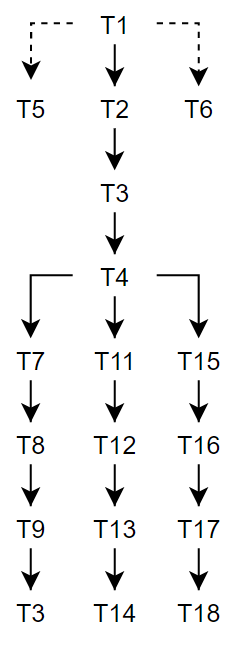
\includegraphics[scale=0.5]{./dependencies.PNG}
    \caption{Dependencies between tasks}
\end{figure}

\vfill

\break

\section{Estimations and Gantt}
As we can see in FIB's documentation \cite{hores}, the TFG corresponds to 18 credits, which have a 30 hours workload each. This means that the total hours spend on the project must be of 540 hours.

With this in mind, we plan a working routine of four hours a day, from the 1st of February to the 15th of June of 2021, what makes a total of 135 days of work, from Monday to Sunday.

To properly organize the tasks over time and to specify their duration, we present the information in a Gantt diagram, that you can see on Figure \ref{figure:gantt}. The tasks duration is sumarized on the Table \ref{table:1}.

\begin{figure}[h!]
    \centering
    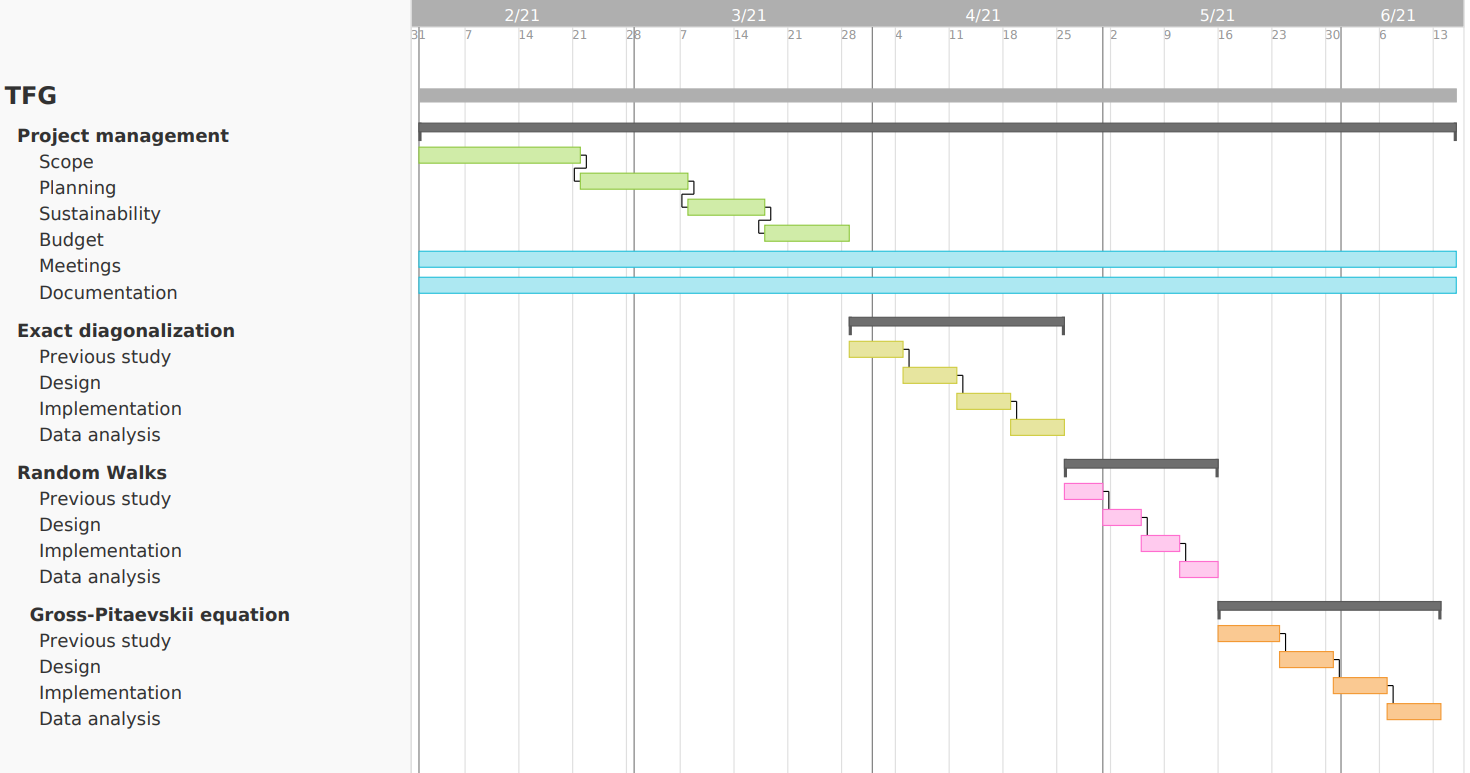
\includegraphics[angle=90, scale=0.45]{./Gantt.PNG}
    \caption{Gantt chart of the tasks of the project}
    \label{figure:gantt}
\end{figure}


\begin{table}[h!]
\centering
\begin{tabular}{|c|c|c|} 

 \hline
 Id & Task name & Hours \\
 \hline
 T1 & Scope & 28 \\
 T2 & Planning & 28 \\
 T3 & Sustainability & 28 \\
 T4 & Budget & 28 \\
 T5 & Meetings & - \\
 T6 & Documentation & - \\
 \hline
 T7 & Exact diagonalization: Previous study & 28 \\
 T8 & Exact diagonalization: Design & 28 \\
 T9 & Exact diagonalization: Implementation & 56 \\
 T10 & Exact diagonalization: Data analysis & 28 \\
 \hline
 T11 & Random walks: Previous study & 28 \\
 T12 & Random walks: Design & 28 \\
 T13 & Random walks: Implementation & 56 \\
 T14 & Random walks: Data analysis & 28 \\
 \hline
 T11 & Gross-Pitaevskii equation: Previous study & 28 \\
 T12 & Gross-Pitaevskii equation: Design & 28 \\
 T13 & Gross-Pitaevskii equation: Implementation & 56 \\
 T14 & Gross-Pitaevskii equation: Data analysis & 28 \\
 \hline
\end{tabular}
\caption{Table to test captions and labels}
\label{table:1}
\end{table}

\section{Risk management: Alternative plans and obstacles}
There are some implicit risks in every project when you plan it in advance. 

The main limitations we can find are about computational cost. We know that exist the algorithms to solve the problems we are tackling, but maybe the cost of solving the systems for a high number of iterations of the fractal is too much for our computers. The more iterations we can do, the more precise our results are going to be. This can lead to a rescheduling of the tasks, as we might need more time to find and implement a more efficient way to solve the equations. 

If this happens we might end up just discarding one of the three studies that we initially planned. 


\section{Budget}
\subsection{Identification of costs}
Referent to this project, we can consider three kinds of costs:
\begin{itemize}
    \item Thesis supervisor: the continuous supervision of a physicist.
    \item Development: the laptop and the main developer work.
    \item Server: energy and rental of the servers to run the simulations.
\end{itemize}

\subsubsection{Thesis supervisor}
This is an interdisciplinary project which involves a lot of specific quantum physics concepts. That is why there appears the need of a physics PHD to supervise and orientate the project.\\

We established a weekly meeting of one hour approximately, that takes place every Tuesday. He also keeps track of my developing process and answers my emails during the week, what can be approximated by on hour of work a week as well.\\

We can see how an investigator at UPC has a monthly salary of 2.313,52€ on the \textit{Taules retributives PDI laboral 2020} \cite{TR}, which implies a salary of 12,85€/h approximately.

\subsubsection{Development}
This is an A modality TFG \cite{TFG_docu}, which implies that is being done by a computer engineering student. 
The economic cost on this process is the usage of his personal laptop, which is a LP gram, that can be found for 1200€ on Amazon \cite{LG}, and the salary of the developer, which we set to be a standard salary of 9€/hour.   

\subsubsection{Server}
All the simulations are run on a server. Some of the simulations need considerable amount of resources, such as memory. That is why we run them on a server with 16 CPUs and 64GB of RAM, which we could rent online for approximately 270€ per month.

\subsection{Cost estimates}
The costs of this project are briefly detailed in Table \ref{table:2}, which summarizes the human resources costs and Table \ref{table:3}, which includes some general costs. All together, leads to a total of 6.798,77€. This cost is divided by tasks on Table \ref{table:4}.

\begin{table}[h!]
\centering
\begin{tabular}{|c|c|c|c|c|c|} 
 \hline
 Profile & Salary & Cost/year & Cost/h & Hours & Cost \\
 \hline
 Thesis supervisor & 32.374,48 & 42.044,78 & 16,69 & 20 & 333,77 \\
 Developer & - & - & 9 & 450 & 4.050 \\
 \hline
 \hline
 Total & & & & & 4.383,77 \\
 \hline
\end{tabular}
 \caption{Human resources costs}
 \label{table:2}
\end{table}


\begin{table}[h!]
\centering
\begin{tabular}{|c|c|c|} 
 \hline
 Concept & Quantity & Cost \\
 \hline
 Developer laptop & 1 & 1.200 \\
 Server & 4,5 & 1.215 \\
 \hline
 \hline
 Total & & 2.415 \\
 \hline
\end{tabular}

 \caption{Resources costs}
 
 \label{table:3}
\end{table}


\begin{table}[h!]
\centering
\begin{tabular}{|c|c|c|} 
 \hline
 Id & Task name & Cost \\
 \hline
 T1 & Scope & 352 \\
 T2 & Planning & 352 \\
 T3 & Sustainability & 352 \\
 T4 & Budget & 352 \\
 T5 & Meetings & 333,77 \\
 T6 & Documentation & - \\
 \hline
 T7 & Exact diagonalization: Previous study & 352 \\
 T8 & Exact diagonalization: Design & 352 \\
 T9 & Exact diagonalization: Implementation & 604 \\
 T10 & Exact diagonalization: Data analysis & 1702 \\
 \hline
 T11 & Random walks: Previous study & 352 \\
 T12 & Random walks: Design & 352 \\
 T13 & Random walks: Implementation & 604 \\
 T14 & Random walks: Data analysis & 1702 \\
 \hline
 T11 & Gross-Pitaevskii equation: Previous study & 352 \\
 T12 & Gross-Pitaevskii equation: Design & 352 \\
 T13 & Gross-Pitaevskii equation: Implementation & 352 \\
 T14 & Gross-Pitaevskii equation: Data analysis & 1702 \\
 \hline
 \hline
 Total &  & 6.798,77 \\
 \hline
\end{tabular}
\caption{Table of cost per tasks}
\label{table:4}
\end{table}



\subsection{Management control and contingency plan}
We have included a contingency based on the renting of the servers for the whole duration of the project, even though we are only going to use them once the development process is done. \\

In case of possible errors on the prediction of costs, we will add a contingency margin of 10\% for human resources costs and generic costs. This equals to an added cost of 679,88€, and leads to a total budget of \textbf{7.478,65€}.


\section{Sustainability}
\subsection{Reflection}
I have been aware for years that computer science can have a negative and positive impact on people's lives, on the environment and on the world in general. That's why I try to always think about the ethic consequences of my actions and not waste resources both in my particular life and on any kind of project I am involved on. I find that society does not give the social and environmental sustainability of projects the importance it deserves. 

In any project it is important to perform a sustainability analysis considering three dimensions: economic, environmental and social. 

\subsection{Economic dimension}
The different aspects of the economic dimension of this project are:
\begin{itemize}
    \item This project has a really reduced budget, as the main developer is a student. 
    \item We have established some strategies to entirely organize this project online, so we do not need any kind of office, what could be and additional cost.
    \item We could analyze the need of the renting of the server for the entire duration of the project, but as this is a research project we are not sure about how long we are going to need it. If we finish earlier we can always stop paying it.
    
\end{itemize}

\subsection{Social dimension}
We state some aspects of the social dimensions as follows: 
\begin{itemize}
    \item If we end up with interesting results, it is very likely that this project evolves in a scientific publication. These means that it contributes to the scientific knowledge as it is a research field that has not been properly explored yet.
    \item Our work can lead to other people getting interested in the study of the behaviour of quantum particles in a different shaped external potentials.
    \item It can also demonstrate and show off how important and successful an interdisciplinary project can be, something really important in a bast range of fields.
    
\end{itemize}


\subsection{Ambiental dimension}
To end up with our sustainability analisis, we explore the abiental aspects of the project:
\begin{itemize}
    \item The resources used to develop this project are the ones stated previously, we do not extract or use any kind of natural resource. We also do not emit or produce anything harmful for the environment.
    \item We do not waste office supplies and we try to cut down to the minimum the amount of it that we use.
    \item The programs that we run on the server are really optimized, to save computation time, and with it, energy. 
\end{itemize}


\break

\addcontentsline{toc}{section}{References}
\begin{thebibliography}{9}

\bibitem{BEC}The Gross-Pitaevskii Equation and Bose-Einstein condensates, J. Rogel-Salazar - 10 January 2013.

\bibitem{boseeinstein} 
Exotic fifth state of matter made on the International Space Station, New Scientist, by Jonathan O’Callaghan - 11 June 2020.

\bibitem{} Dynamical symmetry and breathers in a two-dimensionalbose gas,
R. Saint-Jalm, P. Castilho, E. L. Cerf, B. Bakkali-Hassani, J.-L. Ville, S. Nascimbene,J. Beugnon and J. Dalibard, Phys. Rev.X 9, 021035 - 2019.

\bibitem{} Quantum transport in Sierpinski carpets,
Edo van Veen, Shengjun Yuan, Mikhail I. Katsnelson, Marco Polini, and Andrea Tomadin
Phys. Rev. B 93, 115428 – 21 March 2016.

\bibitem{} Solving Hydrogen atom numerically with 14 lines of Matlab code 
[https://timqian.com/2015/03/04/H-atom-numerical/] - 04 March 2015.

\bibitem{} Fundamental Algorithms in Computational Fluid Dynamics, Thomas H. Pulliam, David W. Zingg, doi:10.1007/978-3-319-05053-9 - 2014.

\bibitem{} Solution of BVPs in electrodynamics by stochastic methods, 2007 IEEE Applied Electromagnetics Conference (AEMC), R. Janaswamy, Kolkata, India, pp. 1-4, doi: 10.1109/AEMC.2007.4638046. - 2007.

\bibitem{hores}FIB-UPC, “Normativa del treball final de grau del grau en enginyeria informàtica de la FIB,” 2012. [Online]. Avaliable:  https://www.fib.upc.edu/sites/fib/files/documents/actes/normativatfg-gei\_document\_final.pdf

\bibitem{TR}Taules retributives del personal docent i investigador laboral Any 2020  [https://www.upc.edu/transparencia/ca/informacio-de-personal/sdg8\_2\_1\_retribuciones\_pdi\_2020-1.pdf]

\bibitem{TFG_docu}Normativa del treball final de grau del grau en Enginyeria Informàtica de la Facultat d’Informàtica de Barcelona [https://www.fib.upc.edu/sites/fib/files/documents/estudis/normativa-tfg-mencio-addicional-gei-br.pdf]

\bibitem{LG}Amazon - LG gram 14Z90N-V-AA78B [https://www.amazon.es/LG-gram-14Z90N-V-AA78B-Ordenador-ultraligero/dp/B0861W8D24/]


\end{thebibliography}

\end{document}
